\documentclass{article}
\usepackage[utf8]{inputenc}
\usepackage[maxcitenames=1,style=numeric]{biblatex}
\usepackage{amsmath}
\usepackage{amssymb}
\usepackage{amsthm}
\usepackage{tcolorbox}
\usepackage{graphicx}
\usepackage{algorithm}
\usepackage{algorithmic}
\usepackage{subfig}
\usepackage{hyperref}
\usepackage{cleveref}
\usepackage{thmtools}
\usepackage{thm-restate}
\usepackage{enumerate}
\usepackage{xcolor}
\usepackage{textgreek}

\topmargin -.5in
\textheight 9in
\oddsidemargin -.25in
\evensidemargin -.25in
\textwidth 7in

\title{Machine Learning based TIR predictor}
\author{}
\date{\today{}}

\bibliography{ref.bib}
\DeclareUnicodeCharacter{2212}{-}
\begin{document}

\maketitle

\section{Introduction}

One of the main tenets of synthetic biology is design, evaluation and standardisation of genetic parts \cite{Brophy2014,Canton2008,Stanton2014}. This is usually done in terms of the Design-Build-Test-Learn (DBTL) cycle, where the given genetic part or organism are continually improved by going through a number of turns of the said cycle. This normally involves designing the DNA sequence in CAD software and then physically testing it in a laboratory. Additionally, computer modelling and prediction of part behaviour based on the designed DNA sequence or design of DNA sequence based on expected function can be used\cite{Yeoh2019,Nielsen2016}. Most of these models are based on either the thermodynamic properties of the involved molecules (DNA, RNA, proteins, etc.) or empirically obtained values describing a relevant to a given design property, like Translation Initiation Rate (TRI) in case of Ribosome Binding Sites (RBS) \cite{Xia1998,Chen2013,Reeve2014}. The biggest limitation for this approach currently is the Learn part of the cycle - there is very limited access to methods and software that can improve designs based on experimental results.\\
According to Reeve \emph{et al.} there are three main RBS calculators, all predicting the TRI based on the thermodynamic properties of the RBS and the ribosome \cite{Seo2013,Na2010,Salis2009}. Predictions from all of these models are relatively good ($R^2 >0.8$), but they come with a number of caveats: i) they rely on calculations of free energies that can be hard to estimate with high precision ii) in general, one of the best ways to improve the models' accuracy is by increasing the number of phenomenons taken into account, but this can lead to paradoxically decreased model accuracy due to accumulation of errors \cite{EspahBorujeni2016} and iii) by using deterministic coefficients to calculate energies one disregards often stochastic nature of processes in the cells which again increases perceived prediction error \cite{Goss1998}. \\
Synthetic biology is currently going through a phase of exponential increase in volume of data produced during experiments \cite{Freemont2019}. New experimental methods heavily relying on advances in automation and microfludics allow unprecedented precision and throughput in data generation. These new data-sets can be combined with data reliant machine learning algorithms to generate new models and predictors for use in synthetic biology, vastly improving the DBTL cycle's performance \cite{Camacho2018}. In the past few years there was a significant uptake of Machine Learning based approaches in synthetic biology. Jervis \emph{et al.} used support vector machine and neural network to optimise production of monoterpenoid in \emph{Esherichia coli} \cite{Jervis2019}. Similarly, Costello \emph{et al.} have used a number of machine learning approaches to analyse time-series multiomics data to predict metabolic pathway behaviour \cite{Costello2018}. There were also successful attempts at using deep learning techniques for analysis of big data-sets \cite{Alipanahi2015,Angermueller2016}. However, the use of machine learning in synthetic biology is still in its infancy and will require additional research to show its full potential. \\
Here we present how machine learning algorithms can be used as a part of the DBTL cycle to predict (Learn) and recommend (Design) variants of RBS with goal of optimization of protein level expression. RBS being one of the key genetic elements controlling protein expression and at he same time having a relatively short sequence is a perfect target for establishing workflows that can be later translated to more complicated systems. We have used Gaussian Process-Upper Confidence Bound and multi-armed Bandits algorithms for prediction and recommendation respectively to analyse and optimise the initiation rates of the designed RBS.

\section{Methods}

\subsection{Plasmid Design}

We have used the pBbB6c-GFP plasmid for all our designs. This plasmid comes with GFP mut3b CDS inducible with addition of IPTG. The original RBS for the GFP CDS was replaced with combination of PCR and isothermal assembly. Primers and the assembly strategy have been generated using the Teselagen DESIGN software (Teselagen Biotechnology).

\subsection{PCR}
PCR amplification of the cloning inserts was done using Q5 High-Fidelity 2X Master Mix (NEB, catalogue no. M0492L). 20 \(\mu\)L reactions were prepared by dispensing each of the 10 \(\mu\)M reverse primers into a well of a 96-well PCR plate using the Labcyte Echo Liquid Handler. A mastermix consisting of polymerase premix, plasmid DNA template, and the single 10 forward primer was prepared by and dispensed by hand. Reactions were run using Touchdown PCR or standard PCR cycling methods in BioRad C1000 thermal cyclers. Then, samples were incubated at 37$^{\circ}$C for 60 minutes, followed by a 20-minute heat inactivation step at 80$^{\circ}$C.
Capillary electrophoresis of PCR products was performed using the Agilent Technologies ZAG DNA Analyzer system. 2\(\mu\)L of each PCR reaction was electrophoresed using the ZAG 130 dsDNA Kit (75-20000bp) or ZAG 110 dsDNA Kit (35-5000bp) (Agilent Technologies, catalogue no. ZAG-110-5000; ZAG-130-5000). ProSize Data Analysis Software (Agilent Technologies) was used to generated gel images from the sample chromatograms and sizes were estimated by reference to the upper and lower DNA markers spiked into each sample and a DNA ladder run in well H12 of each sample plate. 

\subsection{Isothermal DNA Assembly}
Constructs were assembled using NEBuilder HiFi DNA Assembly Master Mix (NEB, catalogue no. E2621L). Samples were incubated at 37$^{\circ}$C for 60 minutes, followed by a 20-minute heat inactivation step at 80$^{\circ}$C. Reactions consisting of the common fragment and the variable fragment were prepared using the Echo acoustic liquid handler, to a final volume of 5 or 10\(\mu\)L . Assemblies were run in the thermal cycler for 1 hour at 50$^{\circ}$C, followed by an infinite hold step at 4$^{\circ}$C.

\subsection{\textit{E. coli} transformation}
The DH5α cell line (Thermo Fisher Scientific, catalogue no. 18265017) was made chemically competent using the Mix & Go \textit{E. coli} Transformation Kit & Buffer Set (Zymo Research, catalogue no. T3001). 20\(\mu\)L of cells was aliquoted into each well of a cold 96-well PCR plate and stored at -80$^{\circ}$C for later use. Plates of cells were thawed on a -20$^{\circ}$C cold block before 3µL of the assembly product was added and mixed using the CyBio FeliX liquid handler. Cells were incubated on a cold block for 2-5 minutes before being plated in a 96 square grid on Omnitrays containing LB (BD, catalogue no. ***) with 34\(\mu\)g/mL chloramphenicol (Sigma, catalogue no. ***). Multiple dilutions of cells in LB were prepared and plated in parallel on Omnitrays in 96 square grid. Plates were incubated overnight at 37$^{\circ}$C.

\subsection{Automated colony picking and culturing}
A Singer Instruments PIXL colony picker was used to select individual colonies from the transformation plates. Each selected colony was used to inoculate 1mL of selective medium in a 2mL square well 96 plate. They were then cultured overnight in 37$^{\circ}$C with shaking (~300rpm).

\subsection{Glycerol stock preparation}
100\(\mu\)L of sterile 80\% (v/v) glycerol and 100\(\mu\)L of overnight culture were combined in the wells of a 96 deep (2mL) round well plate using the CyBio Felix liquid handler. They were then sealed with a 96-well silicon sealing mat and transferred to a -80$^{\circ}$C freezer. 

\subsection{Cuture analysis}
Overnight cultures were started by inoculating 1mL of LB medium supplemented with 34\(\mu\)g/mL chloramphenicol with ~2\(\mu\)L of the glycerol stock in a 96 deep (2mL) round well plate. Cultures were incubated at 37$^{\circ}$C with shaking (~300rpm) for ~17 hours. The following morning, 20\(\mu\)L of overnight culture was added to 980\(\mu\)L of fresh selection medium and precultures were grown at 37$^{\circ}$C with shaking in 2mL round well 96 plate. 
After 90 minutes, two parallel cultures were prepared in flat-bottom clear polystyrene 96-well plates and were induced with 500\(\mu\)M IPTG – one plate of 300\(\mu\)L cultures for flow cytometry analysis (induced with 1.5\(\mu\)L of 0.1M IPTG) and one plate of 200\(\mu\)L cultures for plate reader analysis (induced with 1.0\(\mu\)L of 0.1M IPTG).
•	Cytation 5 acquisition and incubation/shaking settings
•	CytoFLEX S acquisition settings

\subsection{Machine learning experimental design}

To automatically design the RBS sequences in batch using machine learning, we consider two parts: 
1) Design an regression algorithm which takes the RBS sequences as input and returns the predicted TIR scores and the confidence intervals. 
2) Design an online learning approach which recommends the RBS sequences based on the predicted TIR scores and confidence intervals. 
Such online learning approach provides the $\textit{exploitation-exploration balance}$ that we use to control our machine learning process.

With the goal of finding RBS sequences with the largest possible TIR score after a total number of rounds $N$,  we consider our experimental design problem as sequentially optimising an unknown reward function $f: \mathcal{D} \rightarrow \mathbb{R}$, where $\mathcal{D}$ is the set containing all RBS sequence points, and $f(\mathbf{x})$ is the TIR score at $\mathbf{x}$. 
In each round $t$, we choose a set of $m$ points $\mathcal{S}_t \subset \mathcal{D}$ and observe the function values of each points in the selected set $\mathcal{S}_t$, i.e. $y_i = f(\mathbf{x}_i) + \epsilon_i$, for all $i \in \mathcal{S}$, where $\epsilon_i$ is the noise (we assume the noise is following Gaussian distribution with unknown mean and variance). This noise is influenced by the accuracy of the RBS predictor and other experimental interference (e.g. time, temperature, operator, etc.). 

For regression model, we consider the \textit{Gaussian Process Regression (GPR)}.
A Gaussian process regression model \cite{Rasmussen2004} is a Bayesian approach which provides uncertainty measurements on predictions. 
We model $f$ as a sample from a \textit{Gaussian process} $\mathcal{G} \mathcal{P}(\mu(\mathbf{x}), k(\mathbf{x}, \mathbf{x'}))$, which is specified by the mean function $\mu(\mathbf{x})=\mathbb{E}[f(\mathbf{x})]$ and the kernel (or covariance) function $k\left(\mathbf{x}, \mathbf{x}^{\prime}\right)=\mathbb{E}[(f(\mathbf{x})-\left.\mu(\mathbf{x}))\left(f\left(\mathbf{x}^{\prime}\right)-\mu\left(\mathbf{x}^{\prime}\right)\right)\right]$.
Denote the training testing data as $X, X_{*}$, and the training label as $\mathbf{y}$.
Then the posterior of the test points (i.e. predictive distributions) is given by the conditional distribution $\mathbf{f}_\ast | X, \mathbf{y}, X_\ast \sim \mathcal{N}(\bar{\mathbf{f}}_\ast, cov(\mathbf{f}_\ast))$, where
\begin{align}
\overline{\mathbf{f}}_{*} & \triangleq \mathbb{E}\left[\mathbf{f}_{*} \mid X, \mathbf{y}, X_{*}\right]=K\left(X_{*}, X\right)\left[K(X, X)+\alpha^{2} I\right]^{-1} \mathbf{y} \\
\label{Eq: predicted variance in main paper}
\operatorname{cov}\left(\mathbf{f}_{*}\right) &=K\left(X_{*}, X_{*}\right)-K\left(X_{*}, X\right)\left[K(X, X)+\alpha^{2} I\right]^{-1} K\left(X, X_{*}\right) 
\end{align}
%For noisy test targets $\mathbf{y}_\ast$, we can compute the predictive distribution by adding $\alpha^2 I$ to the variance term $cov(\mathbf{f}_\ast)$ in Eq. (\ref{Eq: predicted variance in main paper}).

To represent the RBS sequences and formulate the similarity between sequences, we use the \textit{weighted degree kernel with shift} \cite{ratsch_rase_2005} to specify the kernel function of $GP$.  
The weighted degree kernel with shift extends the spectrum kernel \cite{leslie2001spectrum, ben2008support} 
by considering the positional information and allowing some positional shifts of matching substrings.
The spectrum kernel and the weighted degree kernel with shifts are string kernels, which take two sequences as inputs and outputs a scalar value which represents the similarities between the two sequences. 
We define spectrum kernel firstly,
\begin{align}
        k_\ell^{\text{Spec}}(\textbf{x}, \textbf{x}^\prime) =\left\langle\phi_{\ell}^{\mathrm{Spec}}(\mathbf{x}), \phi_{\ell}^{\mathrm{Spec}}\left(\mathbf{x}^{\prime}\right)\right\rangle = \phi_{\ell}^{\mathrm{Spec}}(\mathbf{x})^T \phi_{\ell}^{\mathrm{Spec}}\left(\mathbf{x}^{\prime}\right).
    \end{align}
 where $\mathbf{x}, \mathbf{x}^\prime$ are two RBS sequences in $\mathcal{D}$ over an alphabet $\Sigma$. We denote the number of letters in the alphabet as $|\Sigma|$. 
$\phi_{\ell}^{\mathrm{spec}}(\mathbf{x})$ maps the sequence $\textbf{x}$ into a $|\Sigma|^\ell$ dimensional feature space, where each dimension is the count of the number of one of the $|\Sigma|^\ell$ possible strings $s$ of length $\ell$. 
Let $X, X^\prime$ be two metrics which include $n$ sequences, and $\Phi_d^{Spec}(X) \in \mathbb{R}^{n \times |\Sigma|^{\ell}}$, then the spectrum kernel over metrics is 
    \begin{align}
         K_\ell^{\text{Spec}}(X, X^\prime) = \Phi_{\ell}^{\mathrm{Spec}}(X) \Phi_{\ell}^{\mathrm{Spec}}\left(X^{\prime}\right)^T.
    \end{align}
The weighted degree kernel with shift is defined upon the spectrum kernel, with flexibility of adjusting the substring length $d$, the start position $l$ and the shift length $s$. WDS kernel counts the match of kmers at corresponding positions in two sequences as shown in the following,
\begin{align}
        k_\ell^{WDS}(\mathbf{x}, \mathbf{x}^\prime) 
        &= \sum_{d=1}^{\ell} \beta_d \sum_{l=1}^{L-d+1} \gamma_l \sum_{s = 0, s + l \leq L}^{S(l)} \delta_s
        \left(k_d^{Spec}(\mathbf{x}_{[l+s:l+s+d]}, \mathbf{x}_{[l:l+d]}^\prime) + (k_d^{Spec}(\mathbf{x}_{[l:l+d]}, \mathbf{x}_{[l+s:l+s+d]}^\prime)\right)\\
        &= \sum_{d=1}^{\ell} \beta_d \sum_{l=1}^{L-d+1} \gamma_l \sum_{s = 0, s + l \leq L}^{S(l)} \delta_s
        \left(\mathbb{I}(\mathbf{x}_{[l+s:l+s+d]} = \mathbf{x}_{[l:l+d]}^\prime) + (\mathbb{I}(\mathbf{x}_{[l:l+d]}= \mathbf{x}_{[l+s:l+s+d]}^\prime)\right),
\end{align}
where $\beta_d = \frac{2(\ell - d + 1)}{\ell(\ell+1)}, \delta_s = \frac{1}{2(s+1)}$, $\gamma_l$ is a weighting over the position in the
sequence, where we choose to use a uniform weighting over the sequences, i.e. $\gamma_l = 1/L$. $S(l)$ determines the shift
range at position $l$. 
%Since the sequences in provided data have the pattern that the core area is different from each other, and other areas are similar. So the kernel for Gaussian Process we are using is the sum of kernels, for core areas we use spectrum kernel with string as input directly, and for other areas we use one-hot encoding and dot product kernel for simplicity.
    
    
%  For recommendations, we consider the \textit{Upper Confidence Bound (UCB)} type algorithms. 
%  As one popular type of the bandit algorithms \cite{lattimore2018bandit}, the UCB type of algorithms are based on the \textit{optimism in the face of uncertainty},
 %provide various approaches to sequential design where an agent adaptively chooses one or more options among several actions based on certain policies. In our work we used the Upper Confidence Bound version of that algorithm, which is based on the \textit{optimism in the face of uncertainty}. The UCB algorithm, as the name suggests,
%  which basically select RBS sequences with the maximum upper confidence bound constructed by the sum of the predicted mean and $n$ standard deviation ($n > 0$), i.e. $\operatorname{argmax}_{\mathbf{x}_i \in \mathcal{D}} \left( \mu_t(\mathbf{x}_i) + \beta_t \sigma_t(\mathbf{x}_i)\right)$,
%     where $\beta_t$ is a hyperparameter balancing the exploitation and exploration, 
%     $\mu_t(\mathbf{x}_i), \sigma_t(\mathbf{x}_i)$ are the predicted mean and standard deviation at round $t$ for the sequence $\mathbf{x}_i$. 

For recommending RBS sequences to label, we consider the Upper Confidence Bound (UCB) algorithm, 
%which is based on the \textit{optimism in the face of uncertainty}, 
selecting RBS sequences with the maximum upper confidence bound at round $t$, i.e.
\begin{align}
\label{Eq: GPUCB}
    \operatorname{argmax}_{\mathbf{x}_i \in \mathcal{D}} \left( \mu_{t-1}(\mathbf{x}_i) + \beta_t \sigma_{t-1}(\mathbf{x}_i)\right),
\end{align}
where $\beta_t$ is a hyperparmeter balancing the exploitation and exploration, 
$\mu_t(\mathbf{x}_i), \sigma_t(\mathbf{x}_i)$ are the predicted mean and standard deviation at round $t$ for the sequence $\mathbf{x}_i$.

Since labelling sequences is time-consuming, it is unrealistic to recommend sequence sequentially (i.e. one-by-one) and waiting for the label for each round.
Therefore we consider recommending sequences in batch and use Gaussian Process Batch Upper Confidence Bound (GP-BUCB) algorithm  \cite{desautels2012parallelizing}.
With batches of size $B$, the feedback mapping is then defined as $fb[t] = \lfloor(t-1) / B\rfloor B$, i.e. 
\begin{align}
    \mathrm{fb}[t]=\left\{\begin{array}{cl}
    0 & : t \in\{1, \ldots, B\} \\
    B & : t \in\{B+1, \ldots, 2 B\} \\
    2 B & : t \in\{2 B+1, \ldots, 3 B\} \\
    & \vdots
    \end{array}\right.
\end{align}


A key property of Gaussian Process regression is that the predictive variance in Eq. (\ref{Eq: predicted variance in main paper}) only depends on observed points (i.e. features), but not on the labels of those observed points. 
So one can compute the posterior variance without actually observing the labels. 
The GP-BUCB policy is to select sequences that
\begin{align}
    \operatorname{argmax}_{\mathbf{x}_i \in \mathcal{D}} \left( \mu_{fb[t]}(\mathbf{x}_i) + \beta_t \sigma_{t-1}(\mathbf{x}_i)\right).
\end{align}
And only update $y_{t^{\prime}}=f\left(\boldsymbol{x}_{t^{\prime}}\right)+\varepsilon_{t^{\prime}} \text { for } t^{\prime} \in\{\mathrm{fb}[t]+1, \ldots, \mathrm{fb}[t+1]\}$ at the end of each batch ($\mathrm{fb}[t]<\mathrm{fb}[t+1]$). 
This is equivalent to sequential GP-UCB with \textit{hallucinated observations} $\boldsymbol{y}_{\mathrm{fb}[t]+1: t-1}=\left[\mu_{\mathrm{fb}[t]}\left(\boldsymbol{x}_{\mathrm{fb}[t]+1}\right), \ldots, \mu_{\mathrm{fb}[t]}\left(\boldsymbol{x}_{t-1}\right)\right]$, while the posterior variance decreases. 


\begin{figure}[t]
    \centering
    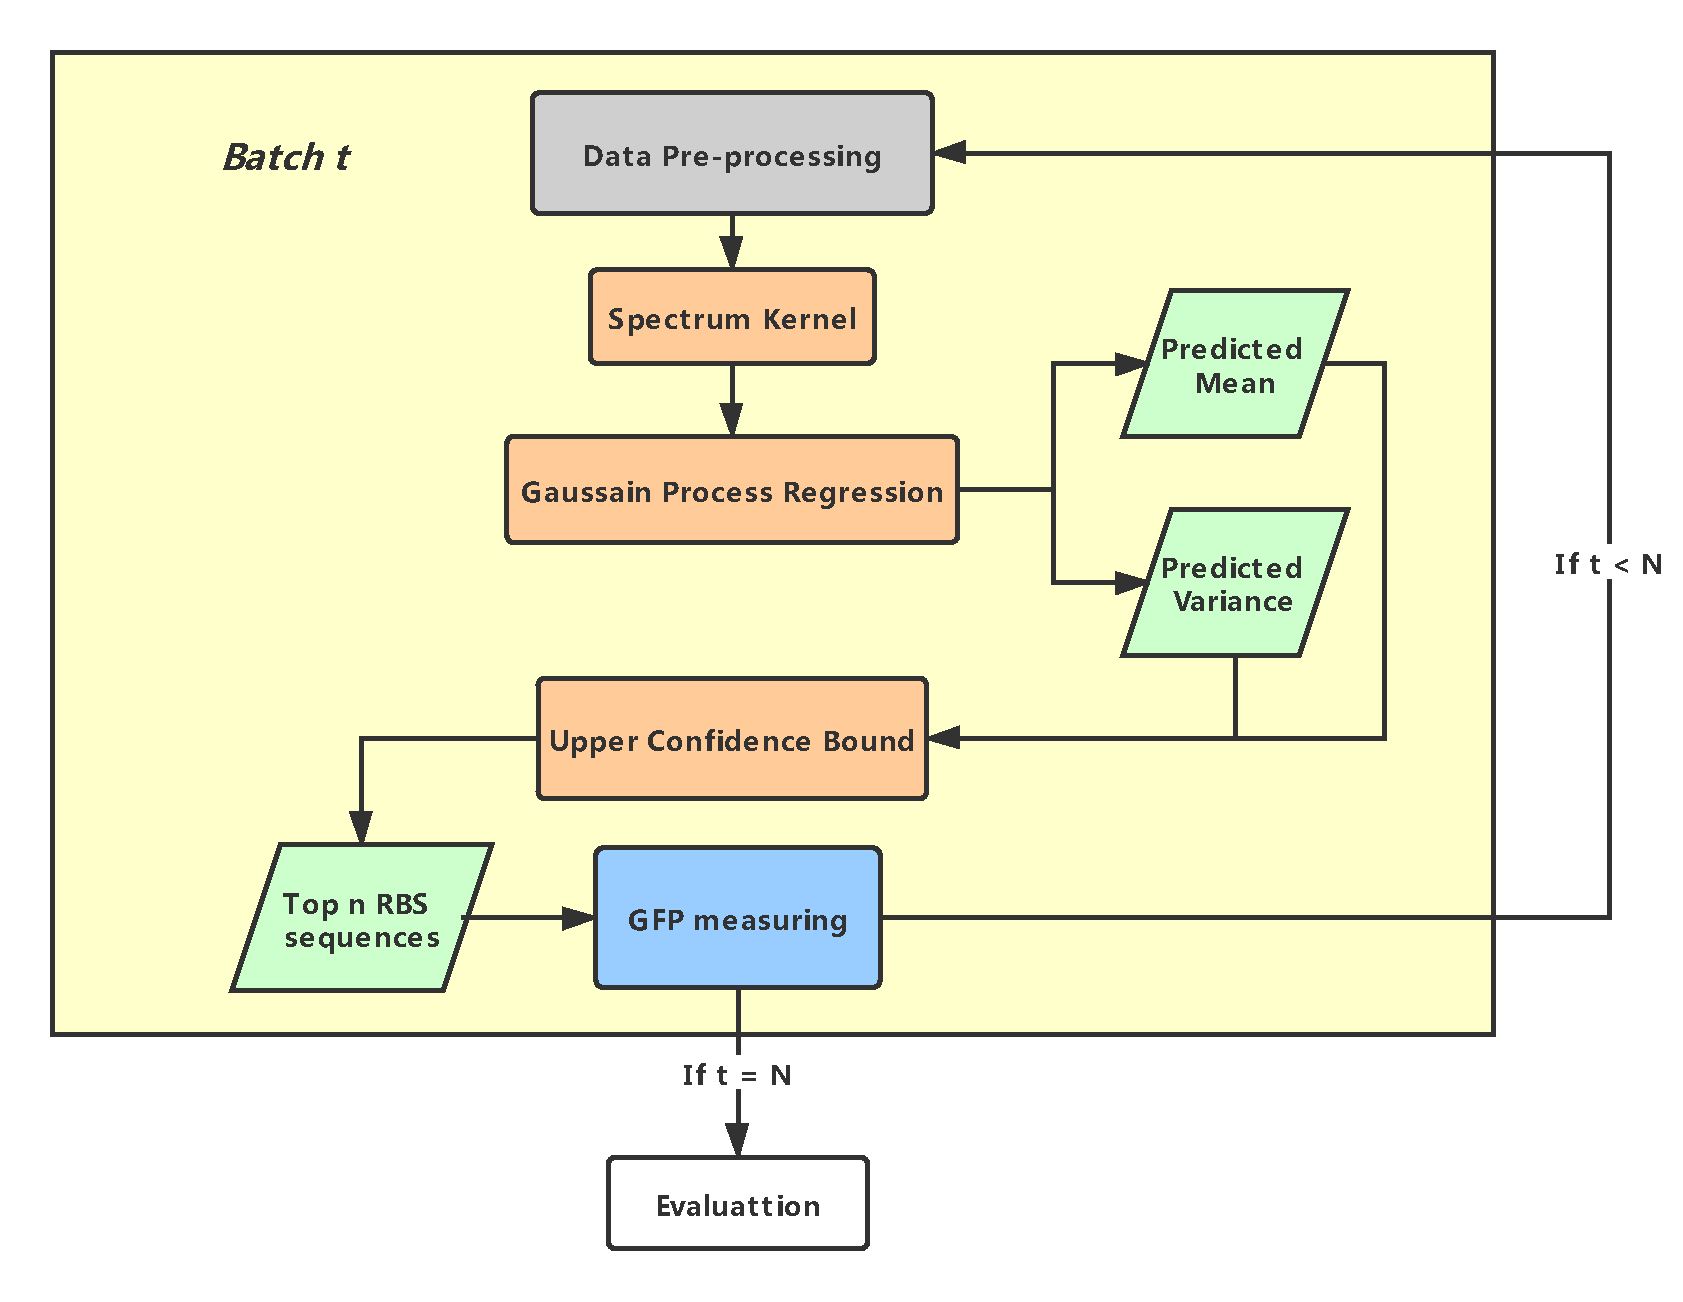
\includegraphics[scale=0.7]{plots/flowchart.pdf}
    \caption{Flowchart of machine learning based experimental design.}
    \label{fig: flowchart of machine learning based experimental design.}
\end{figure}







\section{Results}

Our overall experimental goal was to optimise the translation initiation rate by identifying the set of RBS sequences with top TIR scores while minimising the number of DBTL cycle turns that we had to do. We did this by designing a sequential experimental workflow, where we start with either randomised RBS sequences designed to explore the experimental space (designated round zero since only preexisting, literature data is used for its design) or with RBS sequences recommended by the algorithm (subsequent rounds). The designs were then physically constructed in batches of 90 to fit our automated process (see \textbf{Methods} section). After constructing, the plasmids harbouring the new devices are tested in microplate reader and flow cytometer. The results are then fed back to the algorithm for it to recommend the next round of designs.\\ \textcolor{red}{Figure X} shows the DBTL cycle with the machine learning process emphasised. Our machine learning workflow encompasses two phases of the cycle, namely the LEARN and DESIGN phase. In LEARN phase we use the Gaussian Process algorithm to predict the behaviour of different RBS sequences and in the DESIGN phase we use the multi-armed Bandit algorithm to recommend sequences to be Built and Tested next. Conventionally, the Design phase is considered the beginning of the cycle, however we will start description of our results from the learn phase, which we find a more natural starting point for a machine learning centred workflow.\\


\subsection{LEARN - prediction of RBS performance}
First problem to be tackled was how to embed the sequence to give our RBS sequences numerical form. As we will be using a Gaussian Process for regression we have investigated use of different types of kernels (also called covariances) for embedding \cite{Ben-Hur2008}. The additional, and positive, effect of using kernels is that our data will be moved to a higher-dimensional space, which makes the regression process easier. We compared performance of Dot Product, RBF and a number of string kernels: spectrum, mixed spectrum, weighted degree and weighted degree with shifting \textcolor{red}{Figure Xa}. Since we found that the spectrum kernel performed the best, we have used it in subsequent studies. More specifically, we used a summary of three kernels: spectrum kernel to process the core 6bp and dot product kernel to process the 7bp flanking sequences both upstream and downstream of the core sequence. This approach allowed for good balance between computational complexity and performance.\\
The predictions were made using the Gaussian Process regression (GPR) algorithm. In essence, Gaussian Process is a stochastic (Bayesian) predictor of the shape of a function, which is built based on  perceived similarities between data points (kernels), where not only a mean value, but also probability distribution of the mean is calculated. Such an approach makes GPR well suited to predict biological phenomena which are also highly stochastic. \\
For the zeroth round, since we don't have access to any prior data fitting our design we approximated the predictions using the data from \textcite{jervis2018machine} and the Gaussian Process regression method (see \textbf{Methods} section) \cite{srinivas2012information}. This set contains 113 non-repeated records for 56 unique RBS sequences with the respective TIR. The label values are between 0 - 100,000 and skewed, which is shown in Figure xx. First, we have normalised the label to 0 - 1 using the min-max normalisation. The predictions are shown in \textcolor{red}{Figure Xb}\\
The predictions for next rounds were predicted similarly, but with use of data obtained in previous rounds, visualisation of prediction for the last round of designs is shown in \textcolor{red}{Figure Xc} \\

\subsection{DESIGN of the genetic device}
There is a number of factors that impact the protein expression rate, many of them concerned with how the ribosome recognises and binds to the RBS sequence \cite{Chen1994,Vellanoweth1992}. In \emph{E. coli} the RBS is usually located in the 20 bases upstream of the start codon. The RBS usually has a distinguishable, consensus, core sequence called the Shine-Dalgarno sequence, which in \emph{E. coli} is AGGAGG. Here, we put that 20 bp long sequence into focus with main emphasis being put on the 6bp core region (Figure 1).\\
In our genetic design, the investigated RBS controls expression of the Green Fluorescent Protein (GFP) in its mut3b variant. By controlling expression of a fluorescent protein with the RBS we can quickly assess the perceived TIR by measuring fluorescence of cells harbouring plasmid with the device. Finally, the mRNA is transcribed from an IPTG-inducible promoter pLlacO-1. By making the whole device inducible we can synchronise the start of the expression of the GFP in all the cultures by inducing them at the same optical density (OD\textsubscript{600}) with addition of IPTG.\\
The investigated RBS sequence is 20 bps long with the sequence TTTAAGAAGGAGATATACAT, which is a known high TIR RBS that comes with the pBb series plasmids \cite{Lee2011}. In our design we focus on randomising of the core -8 to -13 (relative to the GFP) nucleotides of the RBS and fix others to be the same as the consensus sequence, i.e. TTTAAGA + NNNNNN + TATACAT. Since for each of the 6 position there are 4 possibilities: A, C, G, T the total variant space is $4^6$ = 4096.\\
Since there was no prior data that we could have used to guide our design for the zeroth round of experiments, we have designed 180 (two times 90) RBS sequences based on the consensus sequence that we expected to give good cover of the experimental space: 

\begin{enumerate}
    \item 60 RBS sequences which are subsequent single nucleotide changes of all 20 nucleotides of the original, consensus sequence. This batch is designed to show us influence of such single nucleotide changes on the overall performance of the RBS and the potential impact of changes made beyond the core part.
    \item 30 RBS sequences that were fully and uniformly randomised (equal probability of choosing either nucleotide for each position) 
    \item 30 RBS sequences randomised based on the position probability matrix (PPM) \textcolor{red}{we need a citation and better explanation for this}  
    \item 60 RBS sequences recommended by our multi armed bandit recommendation algorithm based on the initial literature, as described below.
\end{enumerate}{}

\begin{figure}[t]
    \centering
    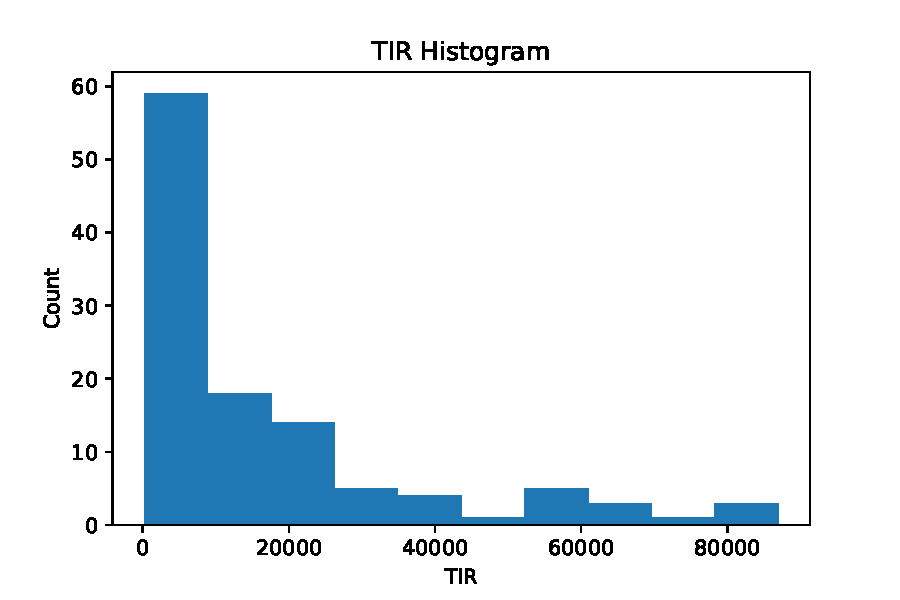
\includegraphics[scale=0.7]{plots/TIR_histogram.pdf}
    \caption{TIR Histogram.}
    \label{fig: TIR Histogram.}
\end{figure}

\begin{enumerate}
    \item RMSE of predictions.
    
    \item Similarity of recommendations. 
    \begin{figure}[t]
    \centering
    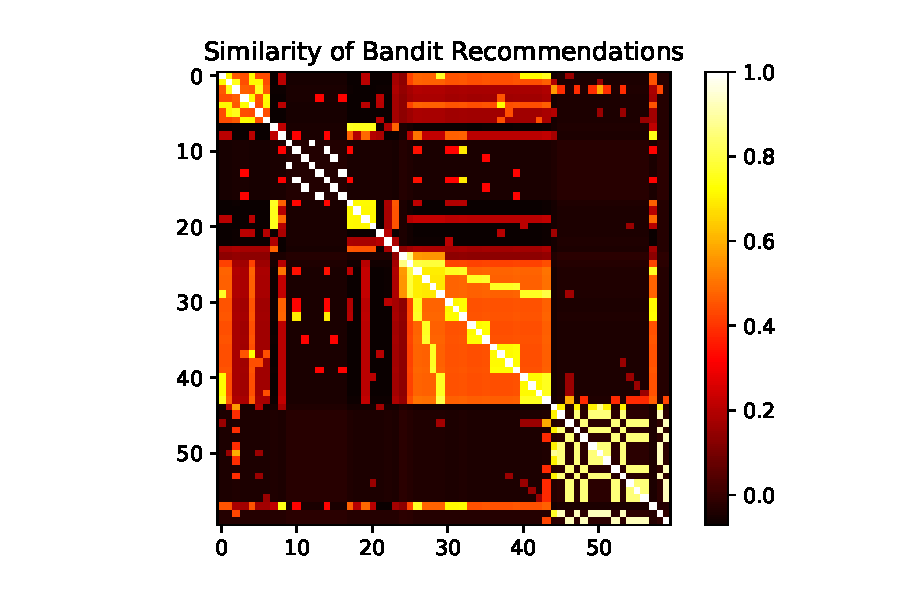
\includegraphics[scale=0.7]{plots/similarity_first_round_recommendation.pdf}
    \caption{TIR Histogram.}
    \label{fig: TIR Histogram.}
\end{figure}
\end{enumerate}{}

The bandit algorithm aims at maximising the reward (output) from testing a limited number of instances from a big pool which cannot be wholly tested due to limited resources (time, computational power, capital). As such, it is very useful in solving problems like the one presented here - a big pool of potential designs, but only limited time and money that can be used for finding the optimal one.\\
In short, the multi-armed bandit algorithm is a stochastic method of probing of the experimental space. In our case we use the Upper Confidence Bound \textcolor{red}{flavour} of the algorithm, which focuses its recommendations on sequences that should give highest TIR based on the probabilities computer by the prediction algorithm (GPR). Another feature of the bandits algorithms is that it balances two approaches: exploration and exploitation. Exploration makes the algorithm to recommend designs that will improve the predictions better, whereas exploitation will recommend designs that focus on delivering the most efficient design the fastest. The two approaches can be controlled with the \textbeta\enspace parameter. We have decided that in the first iterations of the cycle it would be beneficial to skew the algorithm towards the exploration with exploitation taking increasing role in later iterations. One thing of note is that the bandit algorithm is stochastic, that is it exploits the probabilities of given event occurring (in this case RBS having a specific TIR). As such, it pairs naturally with our prediction algorithm, the Gaussian Process, which provides probability based function regression.\\
\\
For rounds beyond the initial, zeroth one, the designs were recommended only by the bandit algorithm based on the data obtained in the previous one, without adding any random designs. In total, three more rounds beyond the initial one have been performed, each with designs recommended by the algorithm. 

\begin{figure}[t]
    \centering
    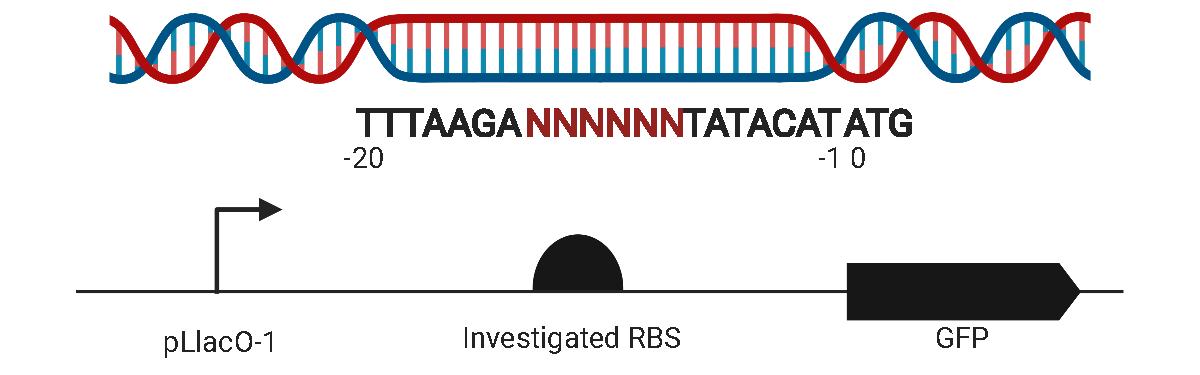
\includegraphics[scale=0.6]{plots/RBS_anatomy.pdf}
    \caption{\textbf{Diagram of the investigated sequence.} The sequence of the investigated RBS is shown with the randomised core sequence in red. The start codon of the GFP coding sequence is also shown with numbers showing relative nucleotide positions. At the bottom a simplified SBOL diagram of the genetic device is shown.}
    \label{fig: Anatomy of the randomized sequence.}
\end{figure}

\subsection{BUILD and TEST}

For the machine learning to work effectively the analysed data-set needs to show two qualities: high relative volume and high quality of data. These two elements don't have a specific definitions, but in general the data-set have to be going into at least hundreds possible data points and you have to cover 5-10\% of that space. And since quality of the obtained data has a direct and strong correlation with quality of the predictions and in effect - recommendations, one need to ensure that the obtained results represent the real value as close as possible.\\
To help us obtain reliable and reproducible results we have employed automation-heavy workflow for our experiments. This way we hope to eliminate a big part of sample-to-sample variation as well as human-introduced variation. Additionally, performing all the procedures directly in 96-well microplate format enabled us to significantly cut down time to prepare our variants.\\
In short, the genetic variations of the RBS were introduced to the plasmids with combination of PCR and isothermal assembly. The plasmids were then transformed and the resulting transformants were tested both using microplate reader and flow cytometry.\\
\textcolor{red}{Figure X} shows the results of the zeroth round.  \\


\textcolor{red}{Figure X} shows the results of the first and subsequent rounds.\\

\subsection{EXIT}
There are two potential points where the exit from the cycle should be considered: i) the optimum solution has been found or ii) depletion of available resources (time and/or money). In our case we have performed a total of four rounds, with performance of the RBSes increasing as seen in \textcolor{red}{Figure X}.\\


\section{Summary}

\newpage

\printbibliography

\clearpage

\appendix
\section*{Appendix}

\section{Gaussian Process Regression}

A \textit{Gaussian process} is a collection of random variables, any finite number of which have a joint Gaussian distribution. 
We define mean function $m(\mathbf{x})$  and covariance function $k(\mathbf{x}, \mathbf{x}^\prime)$ of a real process $f(\mathbf{x})$ as
\begin{align}
    m(\mathbf{x}) &= \mathbb{E}[f(\mathbf{x})]\\
    k(\mathbf{x}, \mathbf{x}^\prime) &= \mathbb{E}[(f(\mathbf{x}) - m(\mathbf{x}))(f(\mathbf{x}^\prime) - m(\mathbf{x}^\prime))].
\end{align}

A Gaussian process is specified by its mean function and convariance function as $f(\mathbf{x}) \sim \mathcal{G} \mathcal{P}\left(m(\mathbf{x}), k\left(\mathbf{x}, \mathbf{x}^{\prime}\right)\right)$.
We consider the case where the observations are noisy, i.e. $\{(\mathbf{x}_i, y_i)| i = 1, \dots, n\}$, where $y_i = f(\mathbf{x}_i) + \epsilon$ with $\epsilon \sim \mathcal{N}(0, \alpha^2)$. 
The Gaussian noise is independent identically distributed, and the prior on the noisy observations is then $\operatorname{cov}\left(y_{p}, y_{q}\right)=k\left(\mathbf{x}_{p}, \mathbf{x}_{q}\right)+\alpha^{2} \delta_{p q}$,
where $\delta_{pq}$ is a Kronecker delta which is one iff $p = q$ and zero otherwise.
It is equivalent to add a diagonal matrix $\alpha^2 I$ on the kernel matrix evaluated on the training points.

For $n_\ast$ test points $X_\ast$, assume the prior over the functions values as a random Gaussian vector $\mathbf{f}_\ast \sim \mathcal{N}(\mathbf{0}, K(X_\ast, X_\ast))$.
Then the joint distribution of the observed target values and the function values at the test points under the prior as 
\begin{align}
    \left[\begin{array}{l}\mathbf{y} \\ \mathbf{f}_{*}\end{array}\right] \sim \mathcal{N}\left(\mathbf{0},\left[\begin{array}{cc}K(X, X)+\alpha^{2} I & K\left(X, X_{*}\right) \\ K\left(X_{*}, X\right) & K\left(X_{*}, X_{*}\right)\end{array}\right]\right)
\end{align}
where $K(X, X_\ast)$ denotes the $n \times n_\ast$ covariance/Kernel matrix evaluated at all pairs of training and testing points, similarly for other kernel matrices.
Then the posterior of the test points (i.e. predictive distributions) is given by the conditional distribution $\mathbf{f}_\ast | X, \mathbf{y}, X_\ast \sim \mathcal{N}(\bar{\mathbf{f}}_\ast, cov(\mathbf{f}_\ast))$, where
\begin{align}
   \overline{\mathbf{f}}_{*} & \triangleq \mathbb{E}\left[\mathbf{f}_{*} \mid X, \mathbf{y}, X_{*}\right]=K\left(X_{*}, X\right)\left[K(X, X)+\alpha^{2} I\right]^{-1} \mathbf{y} \\
   \label{Eq: predicted variance}
   \operatorname{cov}\left(\mathbf{f}_{*}\right) &=K\left(X_{*}, X_{*}\right)-K\left(X_{*}, X\right)\left[K(X, X)+\alpha^{2} I\right]^{-1} K\left(X, X_{*}\right) 
\end{align}
For noisy test targets $\mathbf{y}_\ast$, we can compute the predictive distribution by adding $\alpha^2 I$ to the variance term $cov(\mathbf{f}_\ast)$ in Eq. (\ref{Eq: predicted variance}).
% We now introduce the marginal likelihood (or evidence) $p(\mathbf{y}|X)$, is which the integral of the likelihood times the prior 
% \begin{align}
%     p(\mathbf{y} \mid X)=\int p(\mathbf{y} \mid \mathbf{f}, X) p(\mathbf{f} \mid X) d \mathbf{f}
% \end{align}
The choice of covariance function is critical for the performance of Gaussian process regression, we show the choices of string kernel in next section.


\section{Choices of Kernels}

We consider several string kernels below.

\begin{itemize}
    \item \textit{Spectrum Kernel.}
    \begin{align}
        k_\ell^{\text{Spec}}(\textbf{x}, \textbf{x}^\prime) =\left\langle\phi_{\ell}^{\mathrm{Spec}}(\mathbf{x}), \phi_{\ell}^{\mathrm{Spec}}\left(\mathbf{x}^{\prime}\right)\right\rangle = \phi_{\ell}^{\mathrm{Spec}}(\mathbf{x})^T \phi_{\ell}^{\mathrm{Spec}}\left(\mathbf{x}^{\prime}\right).
    \end{align}
     where $\mathbf{x}, \mathbf{x}^\prime$ are two RBS sequences in $\mathcal{D}$ over an alphabet $\Sigma$. Denote the number of letters in the alphabet as $|\Sigma|$. 
    $\phi_{\ell}^{\mathrm{spec}}(\mathbf{x})$ maps the sequence $\textbf{x}$ into a $|\Sigma|^\ell$ dimensional feature space, where each dimension is the count of the number of one of the $|\Sigma|^\ell$ possible strings $s$ of length $\ell$.  Let $X, X^\prime$ be two metrics which includes $n$ sequences, and $\Phi_d^{Spec}(X) \in \mathbb{R}^{n \times |\Sigma|^{\ell}}$, the spectrum kernel over metrics is 
    \begin{align}
         K_\ell^{\text{Spec}}(\textbf{X}, \textbf{X}^\prime) = \Phi_{\ell}^{\mathrm{Spec}}(X) \Phi_{\ell}^{\mathrm{Spec}}\left(X^{\prime}\right)^T.
    \end{align}
    
    \item \textit{Sum of Spectrum Kernel,} considering weighted sum over different part of the string. 
    
    \item \textit{Mixed Spectrum Kernel,} considering weighted sum over different substring length, with $\beta_d = \frac{2(\ell - d + 1)}{\ell(\ell+1)}$,
        \begin{align}
            k_\ell^{MixedSpec}(\mathbf{x}, \mathbf{x}^\prime) 
            = \sum_{d=1}^{\ell} \beta_d k_d^{Spec}(\mathbf{x}, \mathbf{x}^\prime)
        \end{align}
    \item \textit{Weighted Degree Kernel,} considering positional information. WD kernel counts the match of kmers at corresponding positions in two sequences.
    For sequences with fixed length $L$ and weighted degree kernel consider substrings starting at each position $l = 1, ..., L$, with $\beta_d = \frac{2(\ell - d + 1)}{\ell(\ell+1)}$, \\
    \begin{align}
        k_\ell^{WD}(\mathbf{x}, \mathbf{x}^\prime) 
        &= \sum_{d=1}^{\ell} \beta_d \sum_{l=1}^{L-d+1} \gamma_l k_d^{Spec}(\mathbf{x}_{[l:l+d]}, \mathbf{x}_{[l:l+d]}^\prime)\\
        &= \sum_{d=1}^{\ell} \beta_d \sum_{l=1}^{L-d+1} \gamma_l \phi_d^{Spec}(\mathbf{x}_{[l:l+d]})^T \phi_d^{Spec}(\mathbf{x}_{[l:l+d]}^\prime)\\
        &= \sum_{d=1}^{\ell} \beta_d \sum_{l=1}^{L-d+1} \gamma_l \mathbb{I}(\mathbf{x}_{[l:l+d]} = \mathbf{x}_{[l:l+d]}^\prime),
    \end{align}
    where $\mathbb{I}(\text{true}) = 1$ and 0 otherwise. 
    
    \item \textit{Weighted Degree Kernel With Shift.}
    \begin{align}
        k_\ell^{WDS}(\mathbf{x}, \mathbf{x}^\prime) 
        &= \sum_{d=1}^{\ell} \beta_d \sum_{l=1}^{L-d+1} \gamma_l \sum_{s = 0, s + l \leq L}^{S(l)} \delta_s
        \left(k_d^{Spec}(\mathbf{x}_{[l+s:l+s+d]}, \mathbf{x}_{[l:l+d]}^\prime) + (k_d^{Spec}(\mathbf{x}_{[l:l+d]}, \mathbf{x}_{[l+s:l+s+d]}^\prime)\right)\\
        &= \sum_{d=1}^{\ell} \beta_d \sum_{l=1}^{L-d+1} \gamma_l \sum_{s = 0, s + l \leq L}^{S(l)} \delta_s
        \left(\mathbb{I}(\mathbf{x}_{[l+s:l+s+d]} = \mathbf{x}_{[l:l+d]}^\prime) + (\mathbb{I}(\mathbf{x}_{[l:l+d]}= \mathbf{x}_{[l+s:l+s+d]}^\prime)\right),
    \end{align}
    where $\beta_d = \frac{2(\ell - d + 1)}{\ell(\ell+1)}, \delta_s = \frac{1}{2(s+1)}$, $\gamma_l$ is a weighting over the position in the
    sequence, where we choose to use a uniform weighting over the sequences, i.e. $\gamma_l = 1/L$. $S(l)$ determines the shift
    range at position $l$.
\end{itemize}

\textbf{From kernel to distance}:
$$d(\mathbf{x}, \mathbf{x}^\prime) = \sqrt{k(\mathbf{x}, \mathbf{x}) + k(\mathbf{x}^\prime, \mathbf{x}^\prime) - 2 k(\mathbf{x}, \mathbf{x}^\prime)} $$

\subsection{Normalisation of Kernel}

As part of data pre-processing,
the range of all features should be normalised so that each feature contributes approximately proportionately to the predictive model. 
The kernel matrix is represented by the inner product of the underlying feature vectors, it need to be normalised before using in the downstream regression models. 
Up-scaling (down-scaling) features can be understood as down-scaling (up-scaling) regularizers such that they penalise the features less (more). 

Here we consider two approaches for kernel normalisation: centering and unit norm. 
We will show how to convert the normalisation in terms of feature vectors to normalisation in terms of kernel matrices. 
As defined before, consider $\mathbf{x}, \mathbf{x}^\prime$ are two RBS sequences in $\mathcal{D}$ over an alphabet $\Sigma$.
We denote $\phi(\mathbf{x}_i)$ as a column feature vector of sequence $\mathbf{x}_i$, 
where a feature function $\phi: \mathbf{x} \rightarrow \mathbb{R}^d$. Assume there are totally $n$ sequences in the data $X$ ($n'$ sequences in the data $X'$). 
We illustrate centering and unit norm normalisation below. 

\begin{itemize}
    \item Centering. 
    Define the mean vector $\bar{\Phi}(X) = \frac{1}{n} \sum_{s = 1}^n \phi(\mathbf{x}_s) \in \mathbb{R}^d$, the centered feature vector $\phi^C(\mathbf{x}_i) \in \mathbb{R}^d$ of $\mathbf{x}_i$ is
    \begin{align}
        \phi^{C}(\mathbf{x}_i) = \phi(\mathbf{x}_i) - \bar{\Phi}(X) = \phi(\mathbf{x}_i) - \frac{1}{n'} \sum_{s = 1}^{n'} \phi(\mathbf{x}_s).
    \end{align}
    The corresponding centering kernel value between $\mathbf{x}_i$ and $\mathbf{x}_j$ is then 
    \begin{align}
        k^C(\mathbf{x}_i, \mathbf{x}_j) &= <\phi^C(\mathbf{x}_i), \phi^C(\mathbf{x}_j)>\\
        &= \left( \phi(\mathbf{x}_i) - \frac{1}{n} \sum_{s = 1}^n \phi(\mathbf{x}_s)\right)^T \left( \phi(\mathbf{x}_j) - \frac{1}{n'} \sum_{s' = 1}^{n'} \phi(\mathbf{x}_{s'})\right)\\
        &= \phi(\mathbf{x}_i)^T \phi(\mathbf{x}_j) - \left( \frac{1}{n} \sum_{s = 1}^n \phi(\mathbf{x}_s)\right)^T \phi(\mathbf{x}_j) - \phi(\mathbf{x}_i)^T \left(\frac{1}{n} \sum_{s' = 1}^{n'} \phi(\mathbf{x}_{s'})\right) + \left( \frac{1}{n} \sum_{s = 1}^n \phi(\mathbf{x}_s)\right)^T \left(\frac{1}{n'} \sum_{s' = 1}^{n'} \phi(\mathbf{x}_{s'})\right)\\
        &= k(\mathbf{x}_i, \mathbf{x}_j) - \frac{1}{n} \sum_{s=1}^n k(\mathbf{x}_s, \mathbf{x}_j) - \frac{1}{n'} \sum_{s'=1}^{n'} k(\mathbf{x}_i, \mathbf{x}_{s'}) + \frac{1}{n^2} \sum_{s = 1}^n \sum_{s'=1}^{n'} k(\mathbf{x}_s, \mathbf{x}_{s'})
    \end{align}
    
    \item Unit Norm. Define the ($l_2$) norm of a feature vector $||\phi(\mathbf{x})|| = \sqrt{\sum_{m = 1}^d \phi_d(\mathbf{x})^2} = \sqrt{k(\mathbf{x}, \mathbf{x})} \in \mathbb{R}^+$, then the unit norm feature vector $\phi^{UN}(\mathbf{x}_i) \in \mathbb{R}^d$ of $\mathbf{x}_i$ is 
    \begin{align}
        \phi^{UN}(\mathbf{x}_i) = \frac{\phi(\mathbf{x}_i)}{||\phi(\mathbf{x}_i)||}.
    \end{align}
    The corresponding unit norm kernel value between $\mathbf{x}_i$ and $\mathbf{x}_j$ is then 
    \begin{align}
        k^{UN}(\mathbf{x}_i, \mathbf{x}_j) &= <\frac{\phi(\mathbf{x}_i)}{||\phi(\mathbf{x}_i)||}, \frac{\phi(\mathbf{x}_j)}{||\phi(\mathbf{x}_j)||}>\\
        &= \frac{\phi(\mathbf{x}_i)^T \phi(\mathbf{x}_j)}{||\phi(\mathbf{x}_i)|| \times ||\phi(\mathbf{x}_j)||}\\
        &= \frac{k(\mathbf{x}_i, \mathbf{x}_j)}{\sqrt{k(\mathbf{x}_i, \mathbf{x}_i)  k(\mathbf{x}_j, \mathbf{x}_j)}}
    \end{align}
    
     \item Unit Variance. 
    After the centering and unit norm normalisation, the kernel matrix is unit variance as well. 
    In the following, we show transformations of the unit variance (with centering) normalisation.
    Define the variance vector ${Var}(\Phi(X)) = \frac{1}{n} \sum_{s=1}^n ||\phi(\mathbf{x}_s) - \bar{\Phi}(X)||^2 = \frac{1}{n} \sum_{s=1}^n ||\phi(\mathbf{x}_s) - \sum_{s'=1}^n \left(\phi(\mathbf{x}_s')\right)||^2 = \frac{1}{n} \sum_{s=1}^n  k^C(\mathbf{x}_s, \mathbf{x}_s)  \in \mathbb{R}$, the unit variance feature vector $\phi^{UV}(\mathbf{x}_i) \in \mathbb{R}^d$ of $\mathbf{x}_i$ is
    \begin{align}
        \phi^{UV}(\mathbf{x}_i) = \frac{\phi(\mathbf{x}_i)}{\sqrt{Var(\Phi(X))}}.
    \end{align}
    The corresponding kernel representation is 
    \begin{align}
        k^{UV}(\mathbf{x}_i, \mathbf{x}_j) &= <\frac{\phi(\mathbf{x}_i)}{\sqrt{Var(\Phi(X))}}, \frac{\phi(\mathbf{x}_j)}{\sqrt{Var(\Phi(X'))}}>\\
        &= \frac{\phi(\mathbf{x}_i)^T \mathbf{x}_j}{\sqrt{Var(\Phi(X)) Var(\Phi(\mathbf{X'}))}}\\
        &= \frac{k(\mathbf{x}_i, \mathbf{x}_j)}{\sqrt{ \frac{1}{n} \sum_{s=1}^n  k^C(\mathbf{x}_s, \mathbf{x}_s)  \frac{1}{n} \sum_{s'=1}^{n'}  k^C(\mathbf{x}_{s'}, \mathbf{x}_{s'})}}
    \end{align}
    After centering and unit norm, $ \frac{1}{n} \sum_{s=1}^n  k^C(\mathbf{x}_s, \mathbf{x}_s) = k(\mathbf{x}_i, \mathbf{x}_i)$, which implies that after centering and unit norm, the kernel matrix is already unit variance normalised. 
\end{itemize}
For the Gaussian Process regression, we make of use of two kernel matrices: the kernel function between the training data itself, i.e. $K(X_{train}, X_{train})$; 
the kernel function taking the training data and testing data as inputs, i.e. $K(X_{test}, X_{train})$. 
%It is straightforward to normalise a square kernel which same input, i.e. $n = n'$ and $k(\mathbf{x}_i, \mathbf{x}_i),  k(\mathbf{x}_j, \mathbf{x}_j)$ taken from the diagonal of the matrix. 
%The second one (between train and test) is a little bit tricky. The different is not only that $n \neq n'$. 
We will state two ways of normalise those two kind of matrices:
\begin{itemize}
    \item Normalise training and testing data separately.
    This approach is preferred for most of the machine learning algorithms since it follows the rule we have no information about testing data while training.
    Then for centering, one should subtract the mean vector over the training data for both kinds of matrices.
    For unit norm normalisation, when one calculate $K^{UN}(X_{test}, X_{train})$, the two terms inside of square root: $k(\mathbf{x}_i, \mathbf{x}_i)$ is taken from $K(X_{test}, X_{test})[i,i]$, and $k(\mathbf{x}_j, \mathbf{x}_j)$ is taken from $K(X_{train}, X_{train})[j,j]$.
    
    \item Normalise training and testing data together, i.e. normalise $K(X_{train+test}, X_{train+test})$, then extra the parts we need from the normalised matrix. 
    This approach is suitable for the case one already know the whole testing features. 
    For centering, one should subtract the mean vector over the whole matrix $\Phi(X_{train+test})$. 
    The unit norm normalisation is the same as the previous case. 
\end{itemize}

For our experiment, we fix the design space before training, i.e. the testing features are already known before testing. 
So we choose to normalise the kernel matrix over the training and testing data together,
by first applying centering and then unit norm normalisation. 

\section{Batch Recommendation}

For recommending RBS sequences to label, we consider the Upper Confidence Bound (UCB) algorithm, 
%which is based on the \textit{optimism in the face of uncertainty}, 
selecting RBS sequences with the maximum upper confidence bound at round $t$, i.e.
\begin{align}
\label{Eq: GPUCB}
    \operatorname{argmax}_{\mathbf{x}_i \in \mathcal{D}} \left( \mu_{t-1}(\mathbf{x}_i) + \beta_t \sigma_{t-1}(\mathbf{x}_i)\right),
\end{align}
where $\beta_t$ is a hyperparmeter balancing the exploitation and exploration, 
$\mu_t(\mathbf{x}_i), \sigma_t(\mathbf{x}_i)$ are the predicted mean and standard deviation at round $t$ for the sequence $\mathbf{x}_i$.

Since labelling sequences is time-consuming, it is unrealistic to recommend sequence sequentially (i.e. one-by-one) and waiting for the label for each round.
Therefore we consider recommending sequences in batch and use Gaussian Process Batch Upper Confidence Bound (GP-BUCB) algorithm  \cite{desautels2012parallelizing}.
With batches of size $B$, the feedback mapping $fb[t] = \lfloor(t-1) / B\rfloor B$, i.e. 
\begin{align}
    \mathrm{fb}[t]=\left\{\begin{array}{cl}
    0 & : t \in\{1, \ldots, B\} \\
    B & : t \in\{B+1, \ldots, 2 B\} \\
    2 B & : t \in\{2 B+1, \ldots, 3 B\} \\
    & \vdots
    \end{array}\right.
\end{align}


A key property of Gaussian Process regression is that the predictive variance in Eq. (\ref{Eq: predicted variance}) only depends on observed points (i.e. features), but not on the labels of those observed points. 
So one can compute the posterior variance without actually observing the labels. 
The GP-BUCB policy is to select sequences that
\begin{align}
    \operatorname{argmax}_{\mathbf{x}_i \in \mathcal{D}} \left( \mu_{fb[t]}(\mathbf{x}_i) + \beta_t \sigma_{t-1}(\mathbf{x}_i)\right).
\end{align}
And only update $y_{t^{\prime}}=f\left(\boldsymbol{x}_{t^{\prime}}\right)+\varepsilon_{t^{\prime}} \text { for } t^{\prime} \in\{\mathrm{fb}[t]+1, \ldots, \mathrm{fb}[t+1]\}$ at the end of each batch ($\mathrm{fb}[t]<\mathrm{fb}[t+1]$). 
This is equivalent to sequential GP-UCB with \textit{hallucinated observations} $\boldsymbol{y}_{\mathrm{fb}[t]+1: t-1}=\left[\mu_{\mathrm{fb}[t]}\left(\boldsymbol{x}_{\mathrm{fb}[t]+1}\right), \ldots, \mu_{\mathrm{fb}[t]}\left(\boldsymbol{x}_{t-1}\right)\right]$, while the posterior variance decreases. 


\section{Design Pipeline}

The second round design is based on the first round result, where each sequence has 6 replicates with TIR labels.
We pre-processed the data by taking a logarithm transformation and standardisation of the raw TIR label for each replicates respectively (\textcolor{red}{@Maciej, would you like to describe how raw TIR label is calculated?}). 
After normalisation, each replicate has zero mean and unit variance. 

For prediction, we use Gaussian process regression, with training on all normalised replicates and predicting on the design space (6-base core part design) except known sequences. 
We assume the observation are noisy, where the noise is under centered normal distribution with standard deviation $\alpha$.  
We model the covariance matrix using the weighted degree kernel with shift. 
We normalise the kernel with centering and unit norm in terms of the whole kernel constructed by both first round result and design space. 
The hyperparameter for kernel, including maximum substring length  $l$, maximum shift length $s$, and the noise standard deviation $\alpha$ of Gaussian process model are choose based on 10-repeat 5-fold cross validation. 
We choose $l=6, s= 1, \alpha = 2$ for the second round design. 

For recommendation, we use batch upper confidence bound introduced by GP-BUCB algorithm \cite{desautels2012parallelizing}. 
The upper confidence bound is constructed by predicted mean plus 2 predicted standard deviation.   
We recommend 90 sequences from the design space. 




\section{Intuition behind UCB and visualisation}

\begin{itemize}
    \item Exploitation and exploration explanation.
    \item Visualise coverage by clustering plot.
    \item Table for in-clustering mean and variance.
\end{itemize}

\section{Result analysis}

\begin{itemize}
    \item violinplot.
    \item regression performance plot, table.
    \item kernel matrix plot.
\end{itemize}

\section{Figures}




\end{document}
